% !TeX program = xelatex
\documentclass[9pt,fontset=windows]{ctexbeamer}
\usepackage{tikz}
\usetikzlibrary{shapes.arrows}
\usepackage{multicol}
\usepackage{ragged2e}
\usepackage{color}
\usepackage{amsmath,amssymb,bm}
\usepackage{mathdots}
\usepackage{booktabs}
\usepackage{multirow}
\usepackage{diagbox}
\usepackage{etoolbox}
\usepackage{makecell}
\usepackage{amssymb}
\usepackage{expl3,l3keys2e}
\usepackage{xeCJKfntef}
\usepackage{zhnumber}
\usepackage{fontspec}
\usepackage{caption}
\captionsetup[figure]{font=large,labelfont=large,labelformat=empty}
\usepackage{subcaption}
\usepackage{pifont}
\usepackage{threeparttable}
\usepackage{fontawesome}
\usepackage{progressbar}
\usepackage{lipsum}
\usepackage{xcolor}
\usepackage{soul}
\usepackage{svg}
\usepackage[backend=biber,style=numeric,sorting=none,maxnames=99]{biblatex}
\usepackage{bbding}
\usepackage{pifont}

%% Font setup
\usefonttheme{serif}
\usefonttheme{professionalfonts}
\newCJKfontfamily\SourceHeiHeavy{SourceHanSansCN-Heavy.otf}
\newCJKfontfamily\SourceHeiBold{SourceHanSansCN-Bold.otf}
\newfontfamily\SourceHeiBoldw{SourceHanSansCN-Bold.otf}
\setbeamerfont{frametitle}{size={\fontsize{20}{26}},series={\SourceHeiBold}}
\DeclareMathAlphabet{\mathbcal}{OMS}{cmsy}{b}{n}


%% Color Define
\definecolor{light-gray}{gray}{0.85}
\definecolor{darkcolor}{HTML}{0F4539}
\definecolor{bitlightgreen}{HTML}{0A8F30}
\definecolor{bitgreen}{HTML}{005830}
\definecolor{bitred}{HTML}{A13E0B}
\definecolor{firegold}{HTML}{D4AF37}
\colorlet{accent}{darkcolor}
\colorlet{beamer@blendedblue}{bitgreen}
\setbeamercolor{alerted text}{fg=bitred}
%\setbeamercolor{block title}{use=structure,fg=black,bg=bitlightgreen}


%% Style Setup
\setlength{\fboxsep}{0pt}%
\setlength{\fboxrule}{0.255pt}%
\setbeamertemplate{footline}[frame number]
\setbeamertemplate{bibliography item}[text]
%\setbeamertemplate{frametitle}[default][center]
\setbeamertemplate{navigation symbols}{} % remove the navigation bottons
\setbeamertemplate{frametitle continuation}{}
%\setbeamertemplate{sections in toc}[square]
\newcommand{\CJKhl}[2]{\CJKsout*[thickness=2.5ex,format=\color{#1}]{#2}}
\newcommand{\CJKbanner}[3]{\CJKsout*[thickness=4.5ex,format=\color{#1}]{\color{#2}#3}}
\newcommand{\red}{\color{bitred}}
\newcommand{\green}{\color{bitgreen}}
\newcommand{\lightgreen}{\color{bitlightgreen}}
\newcommand{\mathcolorbox}[2]{\colorbox{#1}{$\displaystyle #2$}}
\tikzset{
	myarrow/.style={
		draw,
		fill=bitred,
		single arrow,
		minimum height=85ex,
		single arrow head extend=1ex
	}
}
\newcommand{\arrowup}{%
	\tikz [baseline=-0.5ex]{\node [myarrow,rotate=90] {};}
}
\newcommand{\arrowdown}{%
	\tikz [baseline=-1ex]{\node [myarrow,rotate=-90] {};}
}
\newcommand{\arrowright}{%
	\tikz [baseline=-1ex]{\node [myarrow,rotate=0] {};}
}

\mode<presentation> {
	\usetheme{Madrid}
	%  \usetheme{boxes}
	%  \usetheme{Warsaw}
	\setbeamercovered{transparent}
	%  \setbeamertemplate{footline}[frame number]
}
\AtBeginSection[]{%
	\begin{frame}%
		\frametitle{目\quad 录}%
		\Large
		\hfill
		\parbox[t]{.95\textwidth}{
			\begin{minipage}[c][0.5\textheight]{\textwidth}
				\textbf{\tableofcontents[currentsection]}
			\end{minipage}
		}
	\end{frame}%
}
\AtBeginSubsection[]{%
	\begin{frame}%
		\frametitle{目\quad 录}%
		\Large
		\hfill
		\parbox[t]{.95\textwidth}{
			\begin{minipage}[c][0.5\textheight]{\textwidth}
				\textbf{\tableofcontents[currentsection,currentsubsection]}
			\end{minipage}
		}
	\end{frame}%
}


%% LOGO
\addtobeamertemplate{frametitle}{}{%
	\begin{tikzpicture}[remember picture,overlay]
		\fill[beamer@blendedblue] (11.5,0.4) circle (0.69cm);
		\fill[firegold] (11.5,0.4) circle (0.62cm);
		\node at (11.5,0.4) {
\includegraphics[height=1.2cm]{./assets/bit.png}};
	\end{tikzpicture}
}


%% BIB
\addbibresource{./pub.bib}
%% ==============================================================
\begin{document}
	\title[中间脚注] % footer mid
	{\huge\SourceHeiBold 论文标题}
	\subtitle{副标题(可空)}
	\author[作者] % footer1
	{
		\begin{table}
			\Large
			{\textcolor{bitgreen}{\rule{9cm}{0.15em}}}\\
			\vspace{8mm}
%			\vspace{-5mm}
			\begin{tabular}{rll}
				{\heiti\bf 答辩人} & : & {\heiti\bf 答辩人姓名}    \\
				{\heiti \bf 邮\quad 箱} & : & {\tt email address}\\
				{\heiti\bf 学\quad 号}  & : & {\tt 0123456789} \\
				{\heiti\bf 导\quad 师}  & : & {\heiti\bf 答辩人导师}\\
				{\heiti\bf 日\quad 期}  & : & {\heiti \today}
			\end{tabular}
			\vspace{-18mm}
		\end{table}
	}
	\institute[北京理工大学]{} % (optional)
	\date[\today]{} % cancel the time indicator in title page but preserve it in the footer.
	
	\begin{frame}% title page
		\vspace{4mm}
		\titlepage
		\centering
%		\vspace{5mm}
		{\heiti 个人主页/开源代码/项目主页}: \hspace{1pt}\faGithub\hspace{1pt} {\color{red}\url{https://github.com/scliubit}}
	\end{frame}
	
	\begin{frame}{目\quad 录}
		\Large
		\heiti
		\vskip 2mm
		\hfill	{ \parbox{.95\textwidth}{\textbf{\tableofcontents[hideallsubsections]}}}
	\end{frame}

	\section{研究背景}
	\begin{frame}[t]
		\frametitle{研究背景}
		\vspace{-3mm}
		\begin{itemize}
			\LARGE\heiti
			\item[$\blacksquare$] 后5G标准化推进,6G预研全面启动
		\end{itemize}
		\vspace{3mm}
		\begin{figure}[t]
			\centering
			\begin{subfigure}{0.3\textwidth}
				\centering
				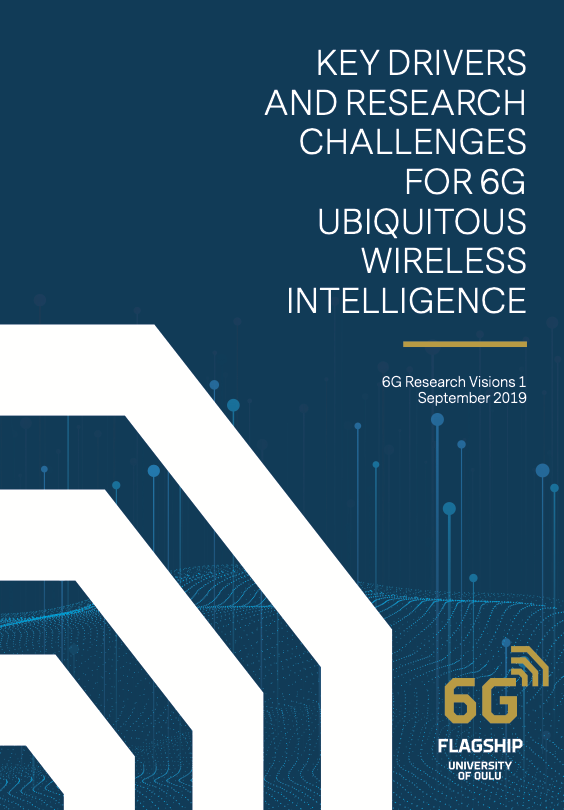
\includegraphics[height=0.5\textheight]{assets/wp6gflagship.png}
				\caption*{\SourceHeiBold \red 首部{\SourceHeiBoldw 6G}白皮书\footnotemark}
				\label{fig:flagshipwp}
			\end{subfigure}
			\begin{subfigure}{0.68\textwidth}
				\centering
				\fbox{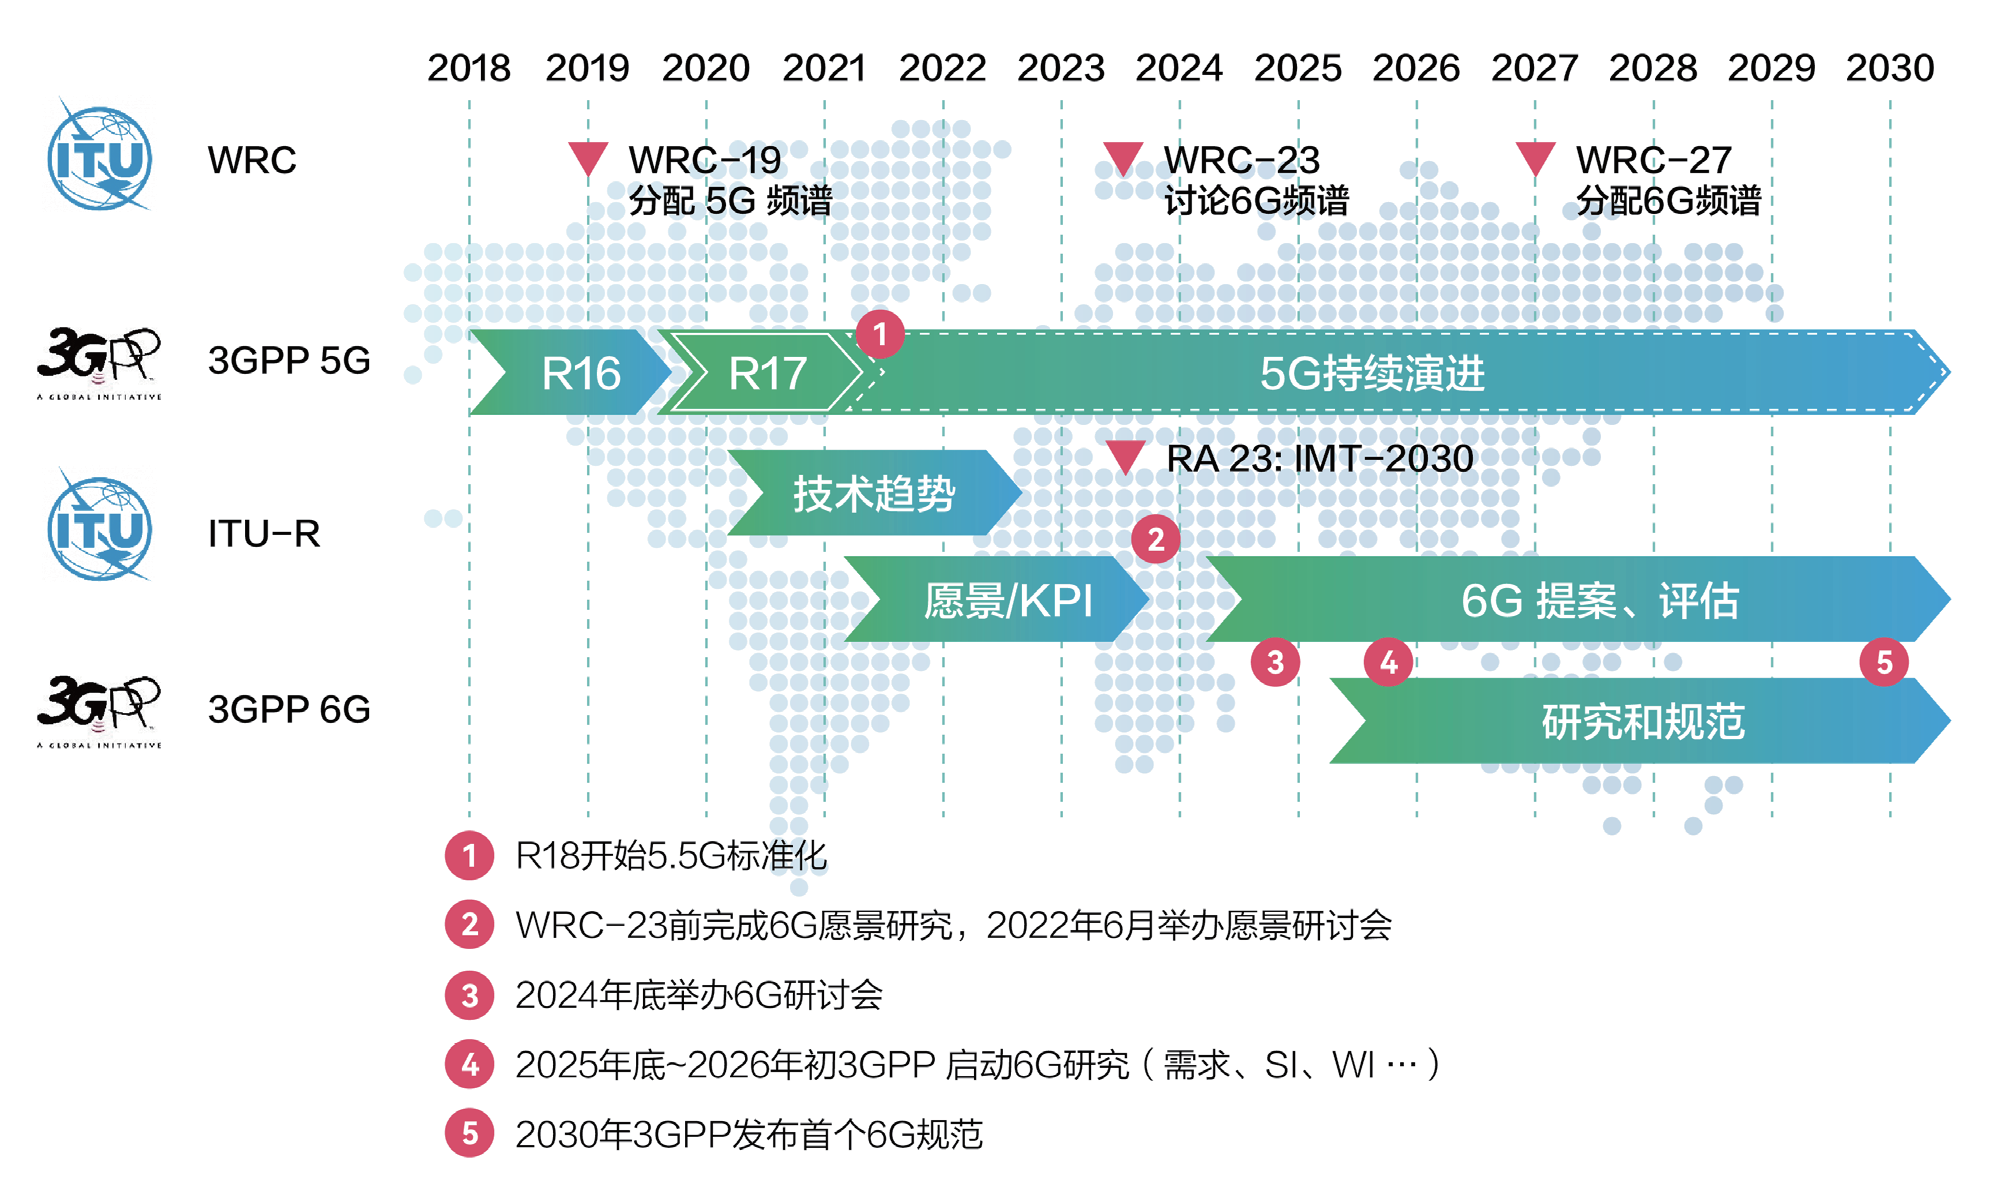
\includegraphics[height=0.5\textheight]{assets/wp6gflagship.jpg}}
				\caption*{\SourceHeiBold \red {\SourceHeiBoldw 6G}标准化时间表\footnotemark}
				\label{fig:hwwp}
			\end{subfigure}
			\vspace{-2mm}
		\end{figure}
		\addtocounter{footnote}{-2}
		\stepcounter{footnote}
		\footnotetext{{\color{bitlightgreen}\bf[WP'19]}\ M. Latva-aho, et al., ``Key drivers and research challenges for 6G ubiquitous wireless intelligence'', Oulu, 2019.}
		\stepcounter{footnote}
		\footnotetext{{\color{bitlightgreen}\bf[WP'22]}\ \textbf{华为技术有限公司, ``6G: 无线通信新征程'', 白皮书}, 2022.}
	\end{frame}
	\begin{frame}[t]
		\frametitle{研究背景}
		\begin{itemize}
			\setlength{\itemsep}{20pt}
			\LARGE\heiti
			\item[$\blacksquare$] 「原神」是由{\red 米哈游}开发的{\SourceHeiBold 动作角色扮演游戏},具有{\SourceHeiHeavy 动漫风格}的{\green 开放世界}环境,采用基于{\lightgreen 抽卡}的{\CJKhl{yellow}{基本免费及道具收费}}制。
			\item[\ding{172}] 游戏剧情于虚构世界的提瓦特大陆上展开,该世界分成七个国家,每个国家都以一种元素为主题,并由一位神明所统治。
			\item[\ding{173}] 游戏剧情的主角为“旅行者”,是一对在无数个世界中旅行的兄妹,因遭遇陌生神明阻拦在提瓦特被迫分离。玩家将扮演旅行者,为了寻找自己失散的唯一血亲,并与派蒙一同游历七国。
		\end{itemize}
	\end{frame}
	\begin{frame}[t]
		\frametitle{研究背景}
		\vspace{-3mm}
		\begin{itemize}
			\LARGE\heiti
			\item[$\blacksquare$] 一种页面布局样例\footnote{{\color{bitlightgreen}\bf[CM'22]}\ Khaled B. Letaief, et al., ``The Roadmap to 6G: AI Empowered Wireless Networks'', {\em IEEE Commun. Mag.}, 2022.}
		\end{itemize}
		\vspace{2mm}
		\begin{figure}
%			\centering
			\begin{subfigure}{0.23\textwidth}
				\centering
				
\includegraphics[width=\textwidth, height=0.13\textwidth]{assets/deepmindlogo.pdf}
			\end{subfigure}\hfill
			\begin{subfigure}{0.23\textwidth}
				\centering
				
\includegraphics[width=\textwidth, height=0.13\textwidth]{assets/deepmindlogo.pdf}
			\end{subfigure}\hfill
			\begin{subfigure}{0.23\textwidth}
				\centering
				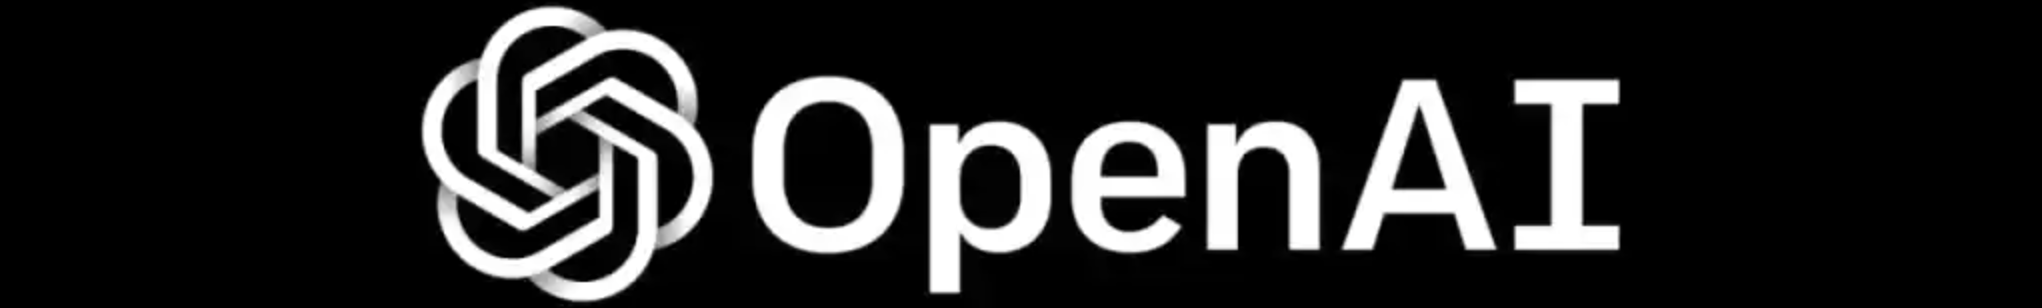
\includegraphics[width=\textwidth, height=0.13\textwidth]{assets/openai.png}
			\end{subfigure}\hfill
			\begin{subfigure}{0.23\textwidth}
				\centering
				
\includegraphics[width=\textwidth, height=0.13\textwidth]{assets/metaai.png}
			\end{subfigure}
			\\\vspace{2mm}
			\begin{subfigure}{0.23\textwidth}
				\centering
				\fbox{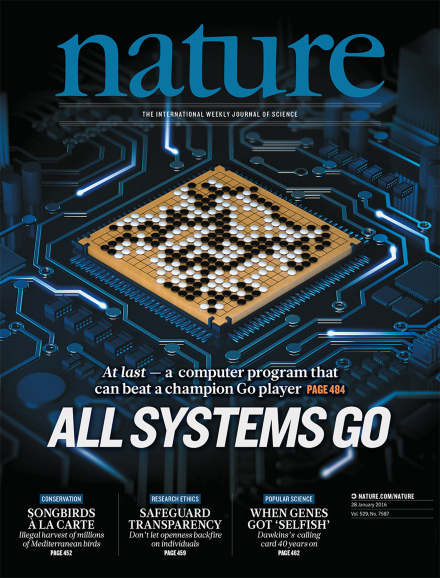
\includegraphics[width=\textwidth,height=1.33\textwidth]{assets/alphago.png}}
				\captionsetup{justification=centering}
				\caption*{\SourceHeiBoldw\red AlphaGo\\2016}
			\end{subfigure}\hfill
			\begin{subfigure}{0.23\textwidth}
				\fbox{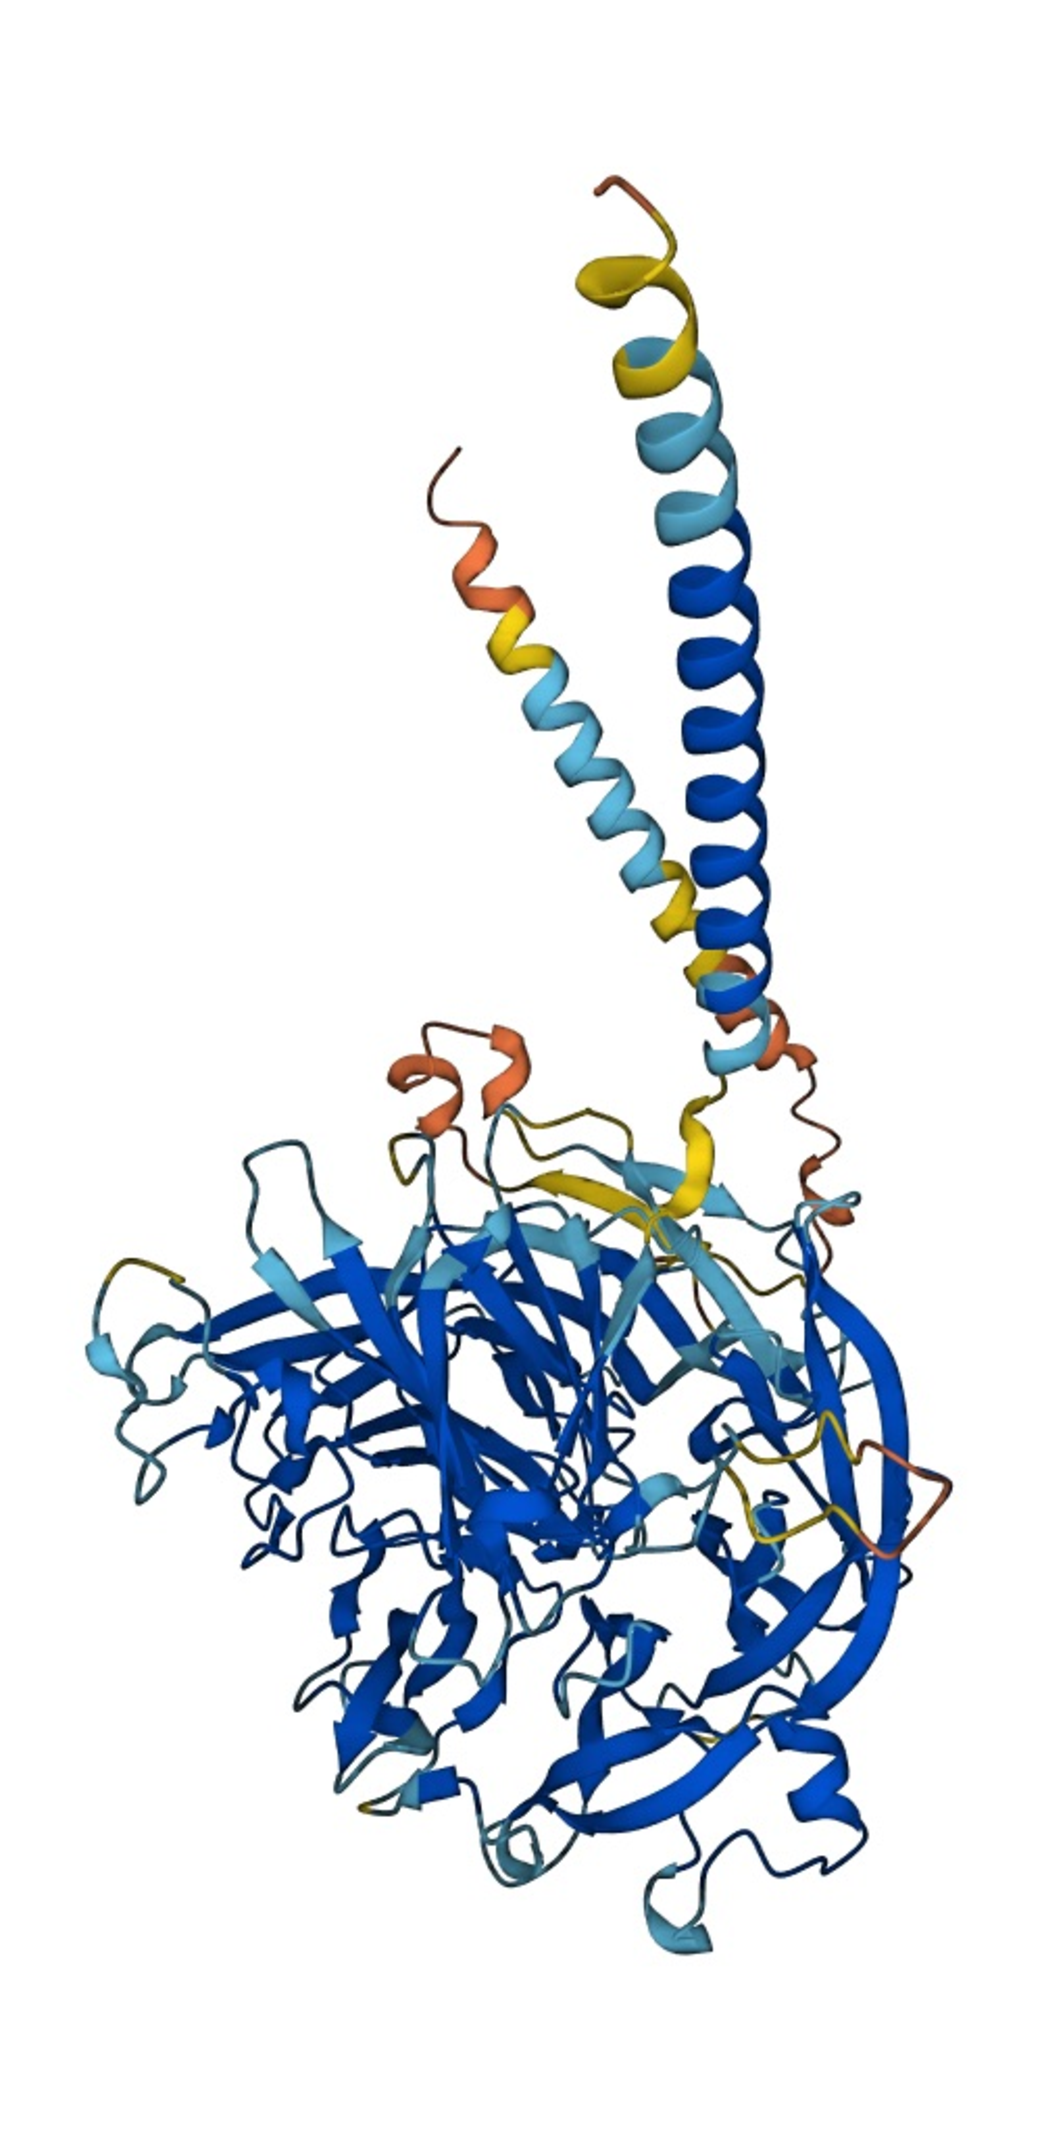
\includegraphics[width=\textwidth,height=1.33\textwidth]{assets/protein.pdf}}
				\captionsetup{justification=centering}
				\caption*{\SourceHeiBoldw\red AlphaFold\\2018}
			\end{subfigure}\hfill
			\begin{subfigure}{0.23\textwidth}
				\centering
				\fbox{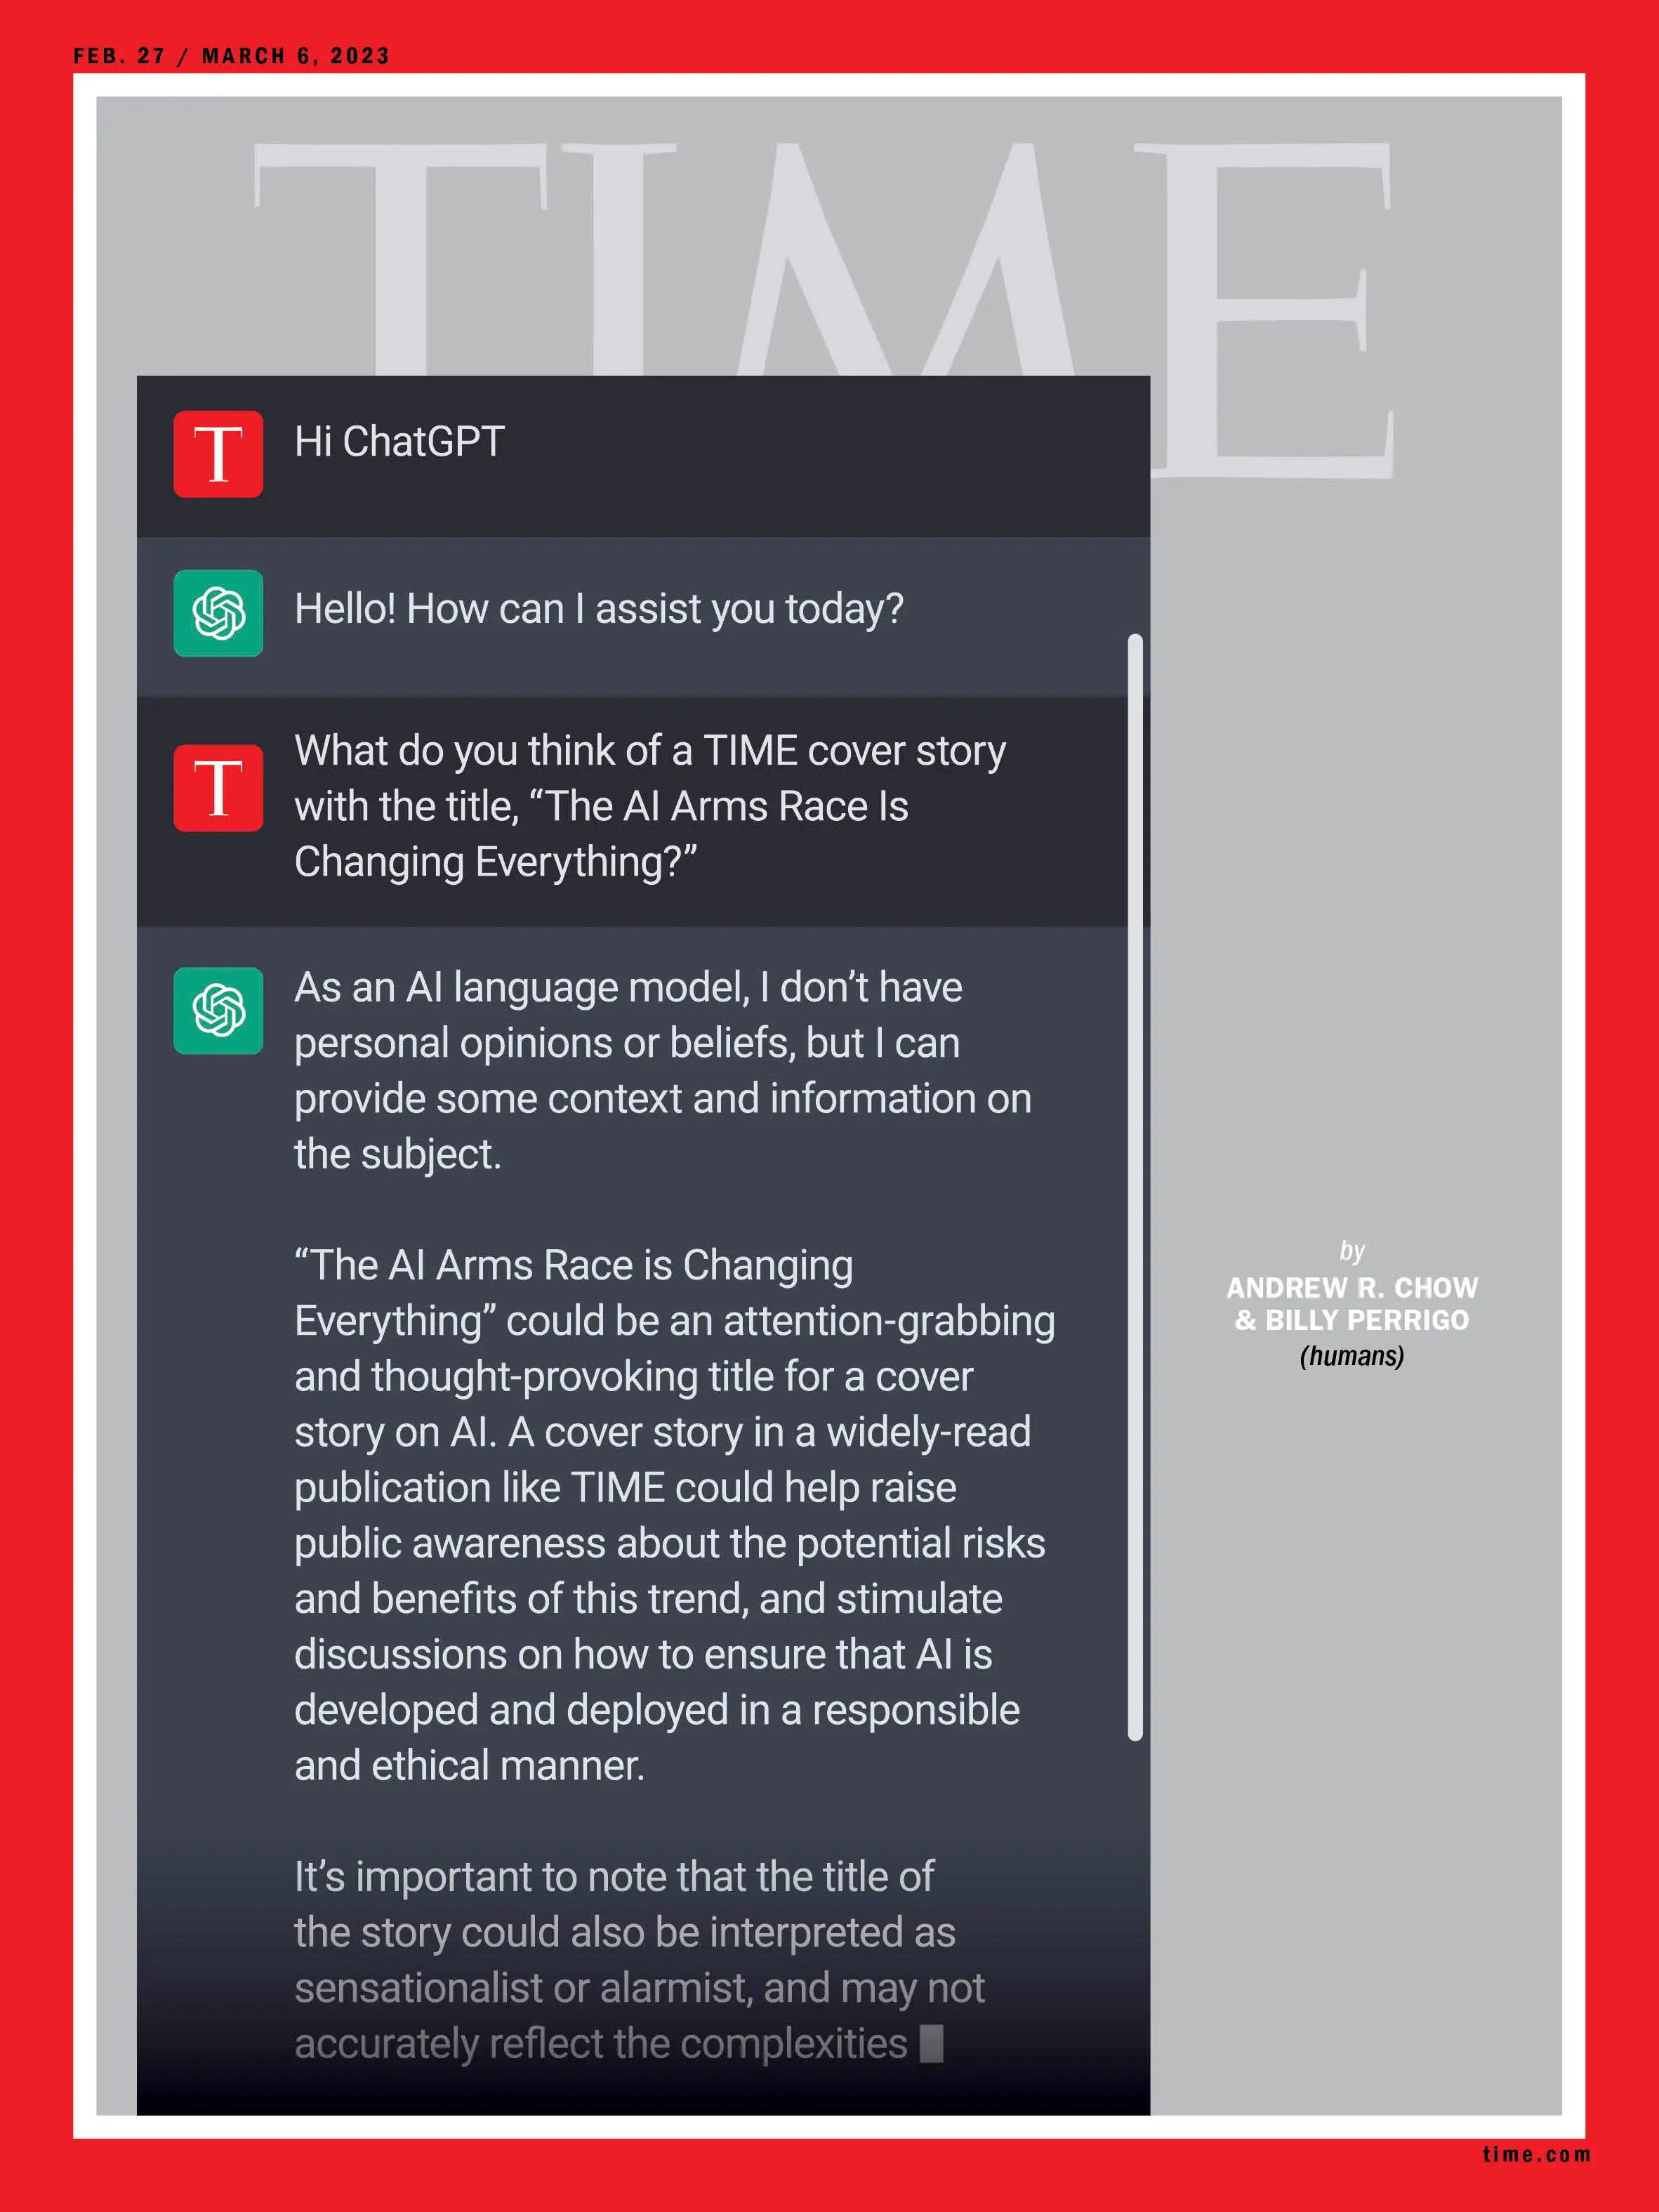
\includegraphics[width=\textwidth,height=1.33\textwidth]{assets/chatgpt.jpeg}}
				\captionsetup{justification=centering}
				\caption*{\SourceHeiBoldw\red GPT-4\\2022}
			\end{subfigure}\hfill
			\begin{subfigure}{0.23\textwidth}
				\centering
				\fbox{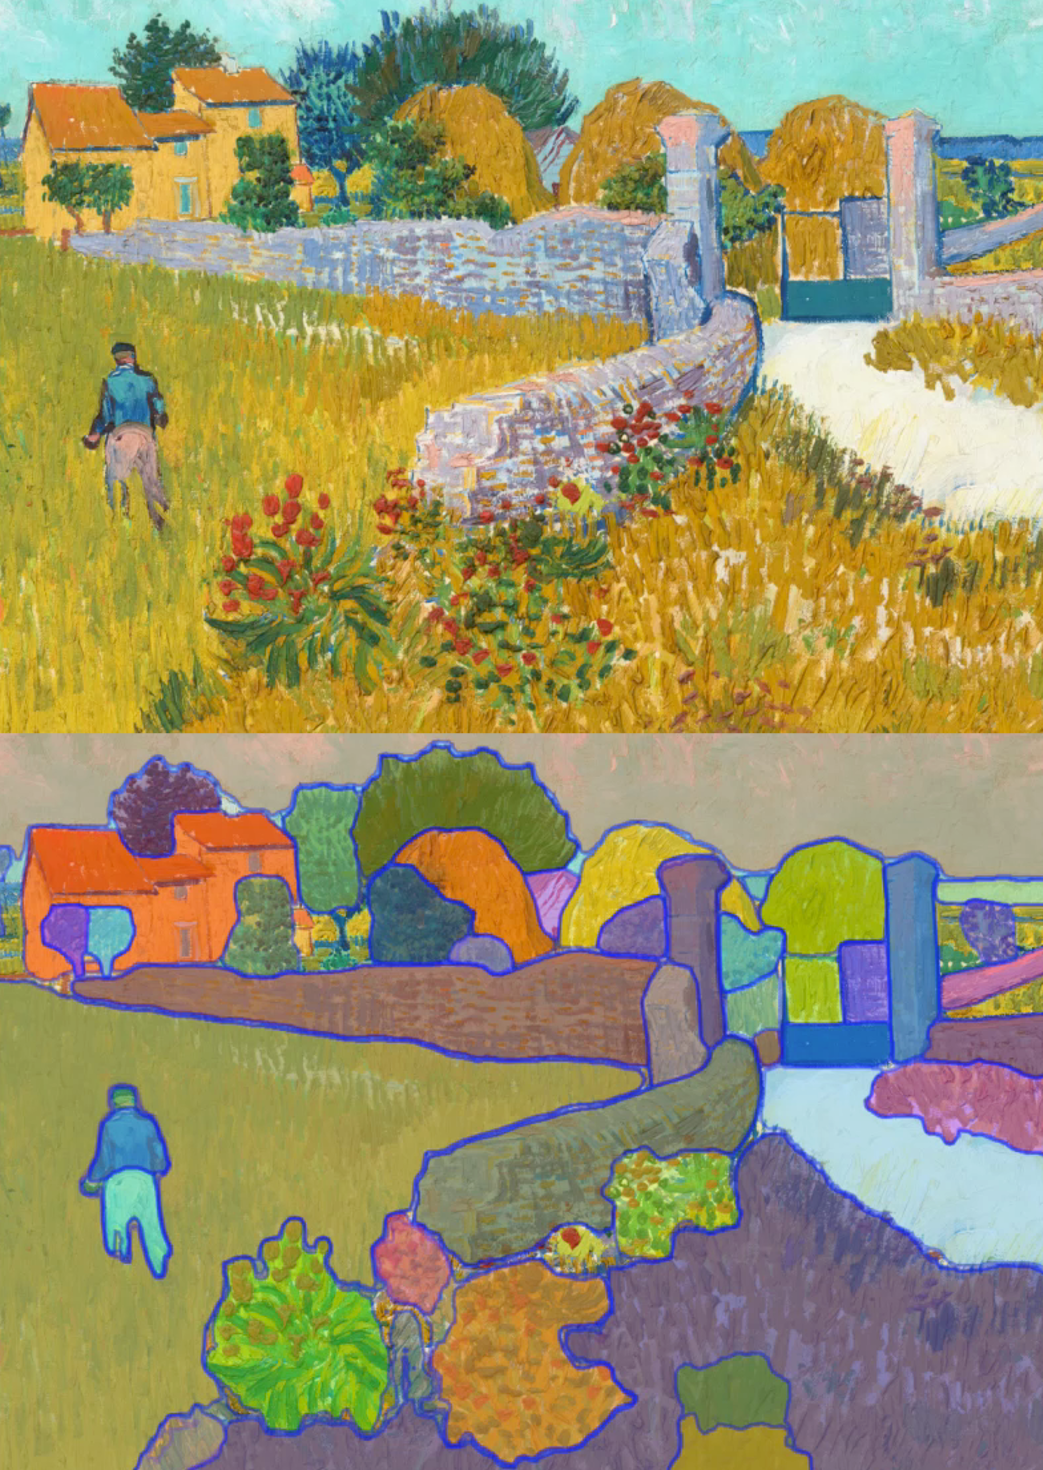
\includegraphics[width=\textwidth,height=1.33\textwidth]{assets/segany2.png}}
				\captionsetup{justification=centering}
				\caption*{\SourceHeiBoldw\red Seg. Anything\\2023}
			\end{subfigure}\\
			\begin{center}
				\vspace{-2mm}
				\arrowright
			\end{center}
		\end{figure}
	\end{frame}
	\begin{frame}[t]
		\frametitle{研究内容与结构安排}
		\begin{figure}
			\centering
			\includegraphics[width=0.7\textwidth, keepaspectratio]{example-image}
		\end{figure}
	\end{frame}
	\section{研究内容}
	\subsection{研究内容1:标题}
	\begin{frame}[t]
		\frametitle{系统模型}
		\vspace{-3mm}
		\begin{itemize}
			\heiti\large
			\item[$\blacksquare$] 稍微加两个公式
			\begin{equation}
				{\bm r}_k=\left({\bm W}_{\mathrm{RF}} {\bm W}_{\mathrm{BB}, k}\right)^H\left({\bm H}_{1, k} \boldsymbol{\Theta} {\bm H}_{2, k} {\bm F}_{\mathrm{RF}} {\bm F}_{\mathrm{BB}, k} {\bm x}_k+{\bm n}_k\right),
				\label{eq:uplinktrans}
			\end{equation}
			\begin{equation}
				\begin{aligned}
					{\bm y}_{u,k}^b={\rm vec}\left(  {\bm y}_{k}^b \left( {\bm s}_{u,k}^b \right)^{\rm H} \right)=\operatorname{vec}\left({\bm Y}_{u,k}^b\right) & =\underbrace{\red \left({\bm F}^b \right)^{\rm T} \otimes\left({\bm W}_{\mathrm{AS}}^b\right)^{\rm H}}_{~} \operatorname{vec}\left({\bm H}_{u,k}\right)+\tilde{\bm n}_k^b \\[-10pt]
					& =\quad\quad\quad\:\:{\red {\bm \Phi}^b}\quad\quad\quad {\bm h}_{u,k}+\tilde{\bm n}_k^b\notag
				\end{aligned}
			\end{equation}
		\end{itemize}
		\begin{figure}
			\centering
			\includegraphics[width=5cm, keepaspectratio]%
			{example-image}
			\caption{\small \bf (a)左半边(b)右半边}
			\label{fig:scenario1}
		\end{figure}
	\end{frame}

	\begin{frame}[t]
		\frametitle{基于xxx的xxx}
	\end{frame}

	\begin{frame}[t]
		\frametitle{基于空间欠采样的信道估计}
		\vspace{-3mm}
		\begin{itemize}
			\heiti\large
			\item[$\blacksquare$] 仿真参数配置
		\end{itemize}
		\begin{figure}
			\centering
			\begin{subfigure}{0.49\textwidth}
				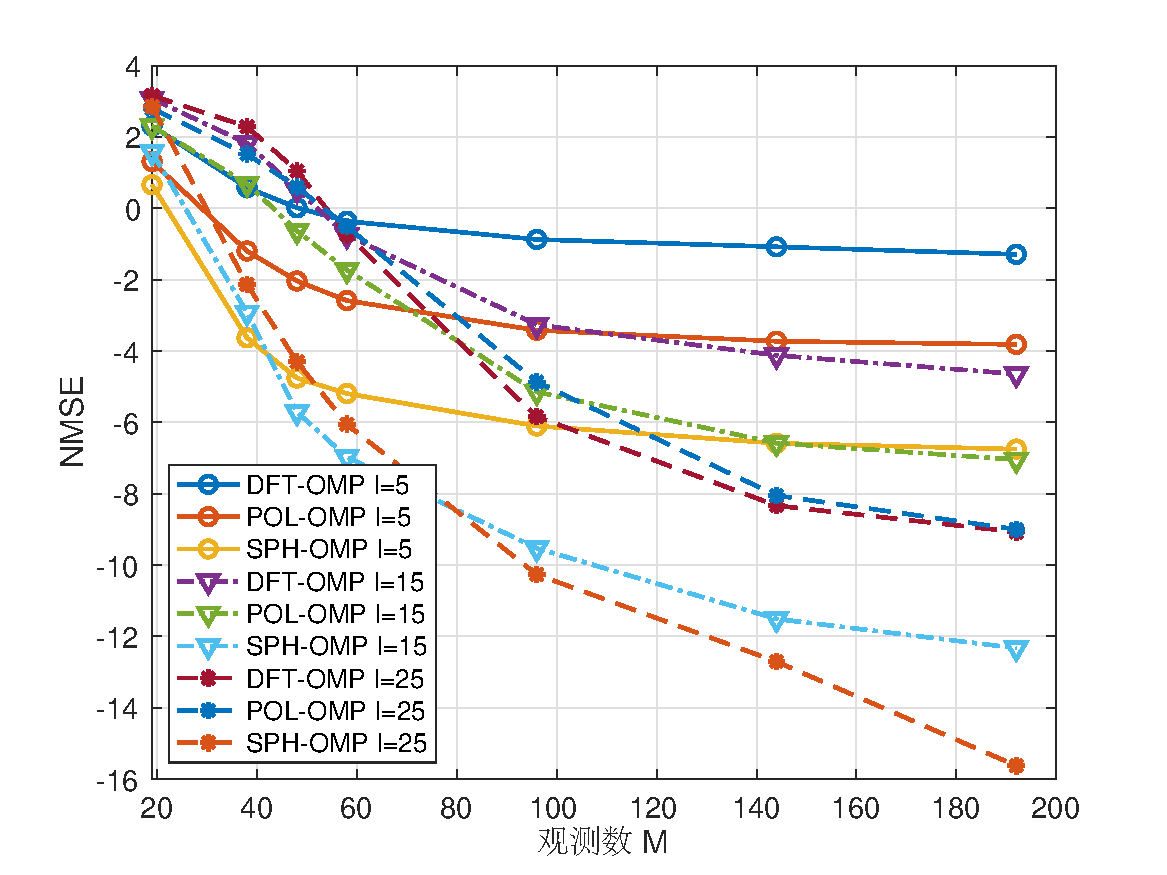
\includegraphics[width=\textwidth]{assets/nf1zh.pdf}
				\caption*{\small\bf (a)图注1}
			\end{subfigure}
			\hfill
			\begin{subfigure}{0.49\textwidth}
				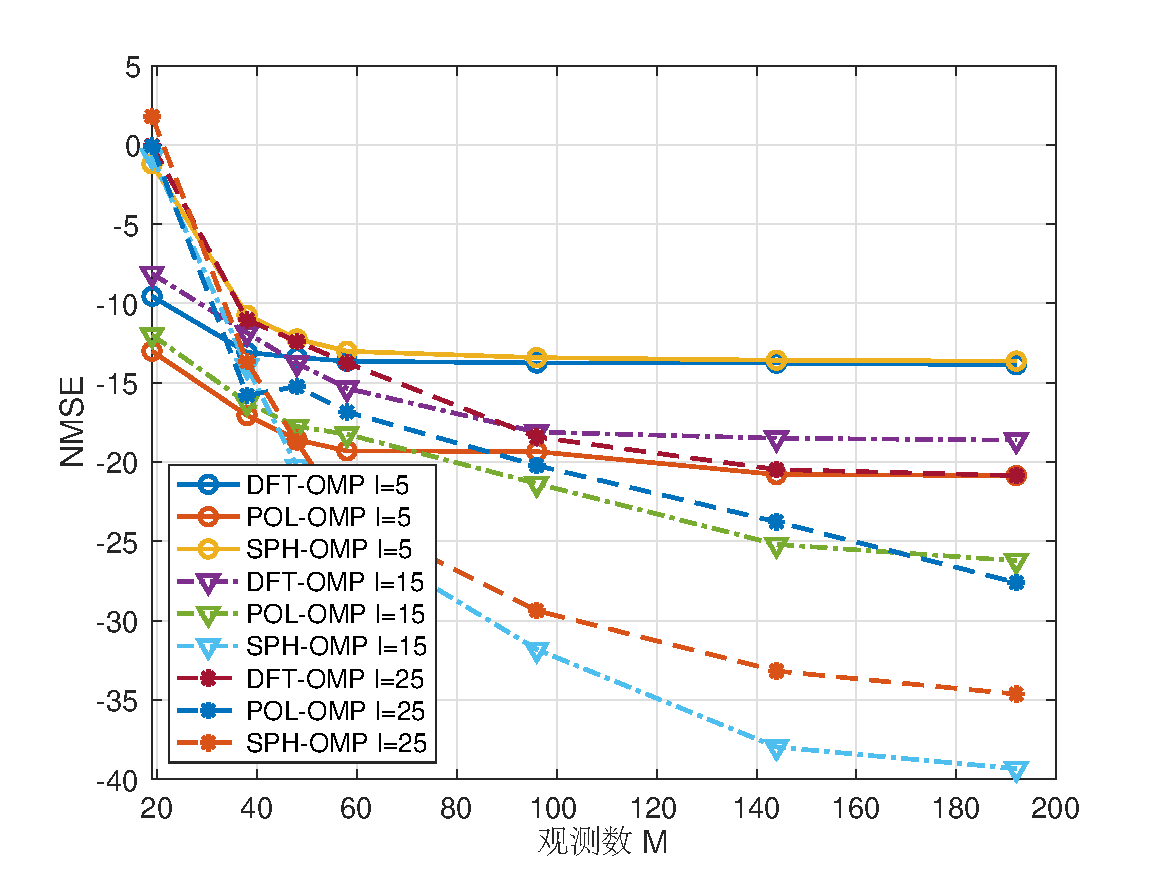
\includegraphics[width=\textwidth]{assets/ff1zh.pdf}
				\caption*{\small\bf (b)图注2}
			\end{subfigure}
		\end{figure}
		\begin{center}
			\LARGE
			\fbox{\SourceHeiBold\color{white}\CJKbanner{bitred}{white}{\quad 这里可以加一个横幅作为性能总结\quad}}
			\vspace{-3mm}
		\end{center}
	\end{frame}

	\begin{frame}[t]
		\frametitle{小结}
		\begin{itemize}
			\setlength{\itemsep}{2mm}
			\heiti\large
			\item[$\blacksquare$] 成果小结
			\item[$\blacksquare$] 分条陈述
			\item[$\blacksquare$] 条理清晰
		\end{itemize}
		\vspace{3mm}
		\begin{block}{{\bf 相关成果}}
			\begin{itemize}
				\item[{[1]}] 这里展示论文/专利等成果,自动悬挂缩进
				\item[{[2]}] 这里展示论文/专利等成果,自动悬挂缩进
				\item[{[3]}] 这里展示论文/专利等成果,自动悬挂缩进
			\end{itemize}
		\end{block}
	\end{frame}
	
	\subsection{研究内容2:标题}

	\subsection{研究内容3:标题}

	\section{总结展望}
	\begin{frame}
		\frametitle{工作总结}
		\begin{itemize}
			\heiti\Large
			\setlength{\itemsep}{10pt}
			\item[$\blacksquare$] 研究内容1
			\item[$\blacksquare$] 研究内容2
			\item[$\blacksquare$] 研究内容3
		\end{itemize}
	\end{frame}
	\begin{frame}
		\frametitle{未来展望}
		\begin{itemize}
			\heiti\Large
			\setlength{\itemsep}{10pt}
			\item[$\blacksquare$] {\SourceHeiBold 研究方向1}: 简介
			\item[$\blacksquare$] {\SourceHeiBold 研究方向2}: 简介
			\item[$\blacksquare$] {\SourceHeiBold 研究方向3}: 简介
		\end{itemize}
	\end{frame}
	\begin{frame}[t]
		\frametitle{盲审意见总结}
		\vspace{-2mm}
		\begin{alertblock}{\heiti 1. 问题1}
			\heiti 做出的修正做出的修正做出的修正做出的修正做出的修正做出的修正做出的修正做出的修正做出的修正做出的修正做出的修正做出的修正做出的修正做出的修正做出的修正做出的修正做出的修正做出的修正做出的修正做出的修正做出的修正做出的修正
		\end{alertblock}
		\vspace{3mm}
		\begin{alertblock}{\heiti 2. 问题2}
			\heiti 做出的修正做出的修正做出的修正做出的修正做出的修正做出的修正做出的修正做出的修正做出的修正做出的修正做出的修正做出的修正做出的修正做出的修正做出的修正做出的修正做出的修正做出的修正做出的修正做出的修正做出的修正做出的修正
		\end{alertblock}
		\vspace{3mm}
		\begin{alertblock}{\heiti 3. 问题3}
			\heiti 做出的修正做出的修正做出的修正做出的修正做出的修正做出的修正做出的修正做出的修正做出的修正做出的修正做出的修正做出的修正做出的修正做出的修正做出的修正做出的修正做出的修正做出的修正做出的修正做出的修正做出的修正做出的修正
		\end{alertblock}
	\end{frame}
	\section{成果列表}
	\begin{frame}[t,allowframebreaks]
		\frametitle{成果列表}
		% add your own pubs
		\nocite{myCiteKey,myCiteKey2,dummy:1,dummy:2}
		\printbibliography
	\end{frame}
	
	{\usebackgroundtemplate{
\includegraphics[width=\paperwidth]{./assets/lastpagem.jpg}}
		\begin{frame}
			\fontsize{22pt}{26pt}\selectfont
			\SourceHeiHeavy
			\color{bitred}
			\vspace{7cm}
			\begin{center}
%				\bf
				\hspace{1.5cm}感谢各位专家\quad 敬请批评指正\bf! \\ \hspace{1.5cm}Q \& A
			\end{center}
		\end{frame}
	}
\end{document}